\chapter{Installing and configuring Spark locally}
\par In this section we are going to use Spark locally on the ubuntu VM created previously. We will run
Spark on Hadoop YARN. YARN will thus take care of the management of resources for the triggering and
execution of Spark Jobs. 
%Intro\footnotemark\\
\begin{spacing}{1.2}
%note en bas de page
\section{Downloading and Extracting files}

\par Let's start as always by checking the status of the machine
\\
\begin{figure}[!htb] 
\begin{center} 
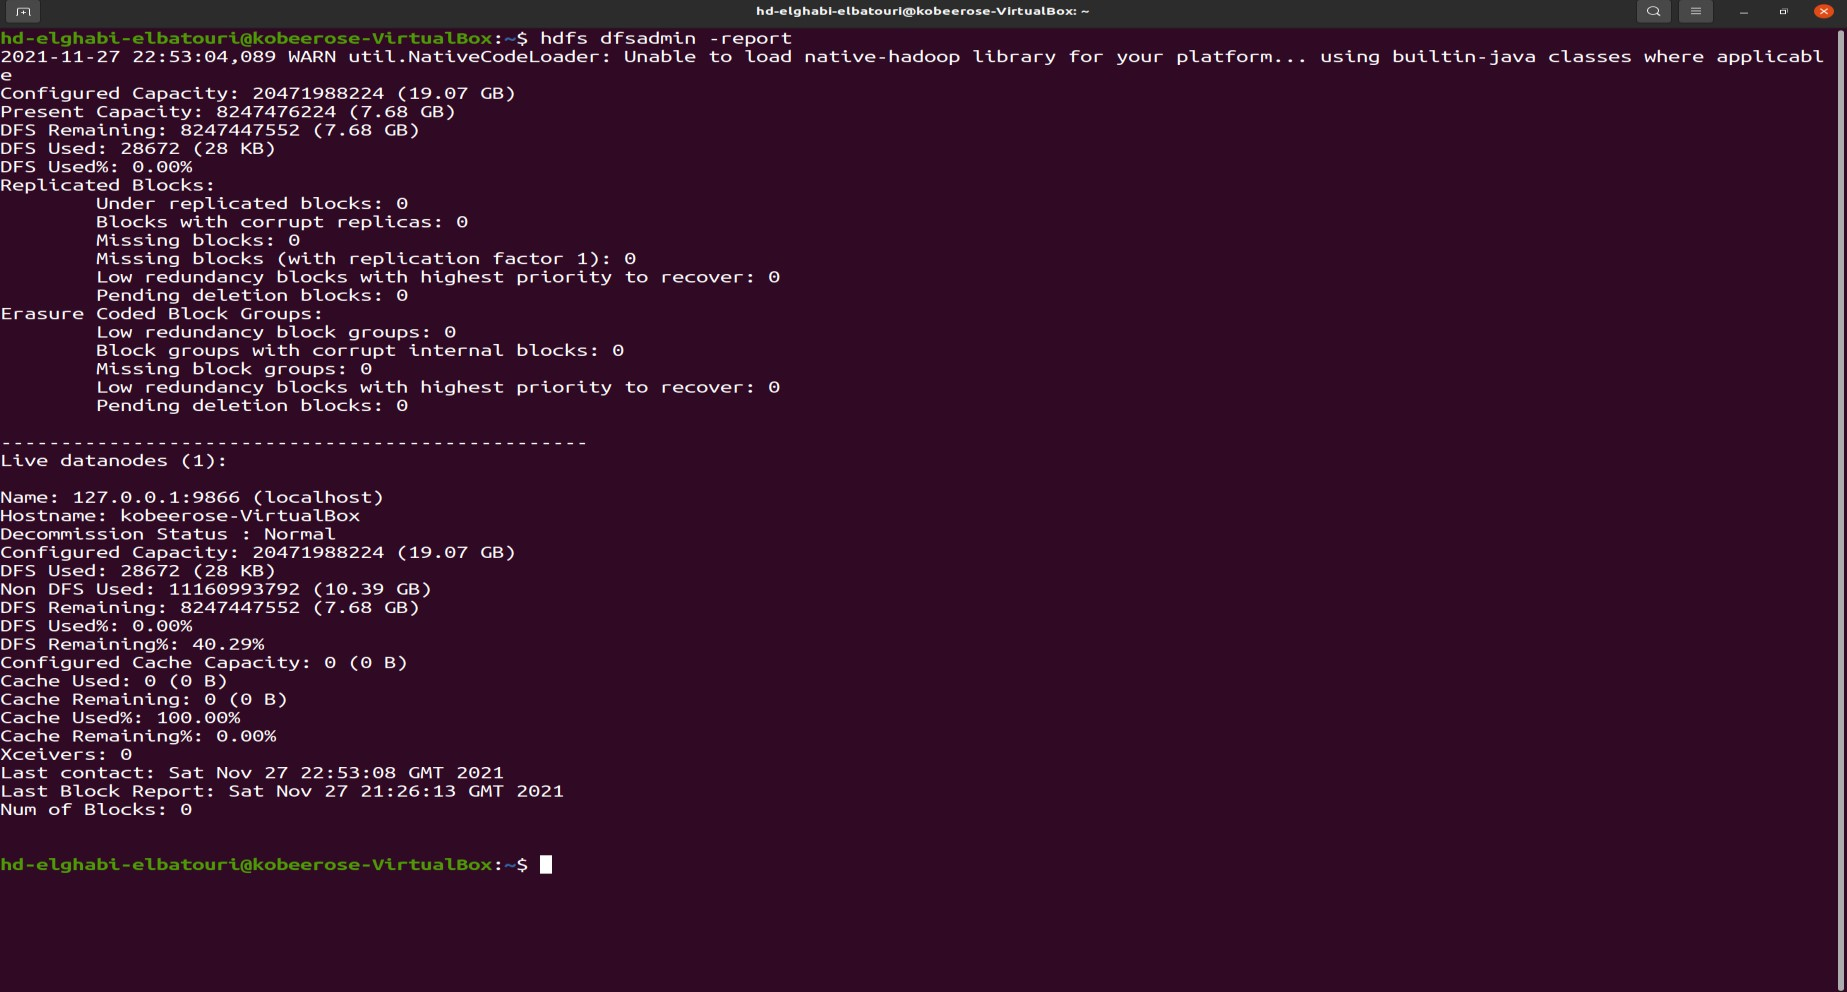
\includegraphics[width=1\linewidth]{Big_Data/Spark/Spark Installation & Configuration/Live datanode.jpg} 
\end{center} 
\caption{caption} 
\end{figure} 
\FloatBarrier



\par After downloading the source files, we will extract them in the download folder.
\\
\begin{figure}[!htb] 
\begin{center} 
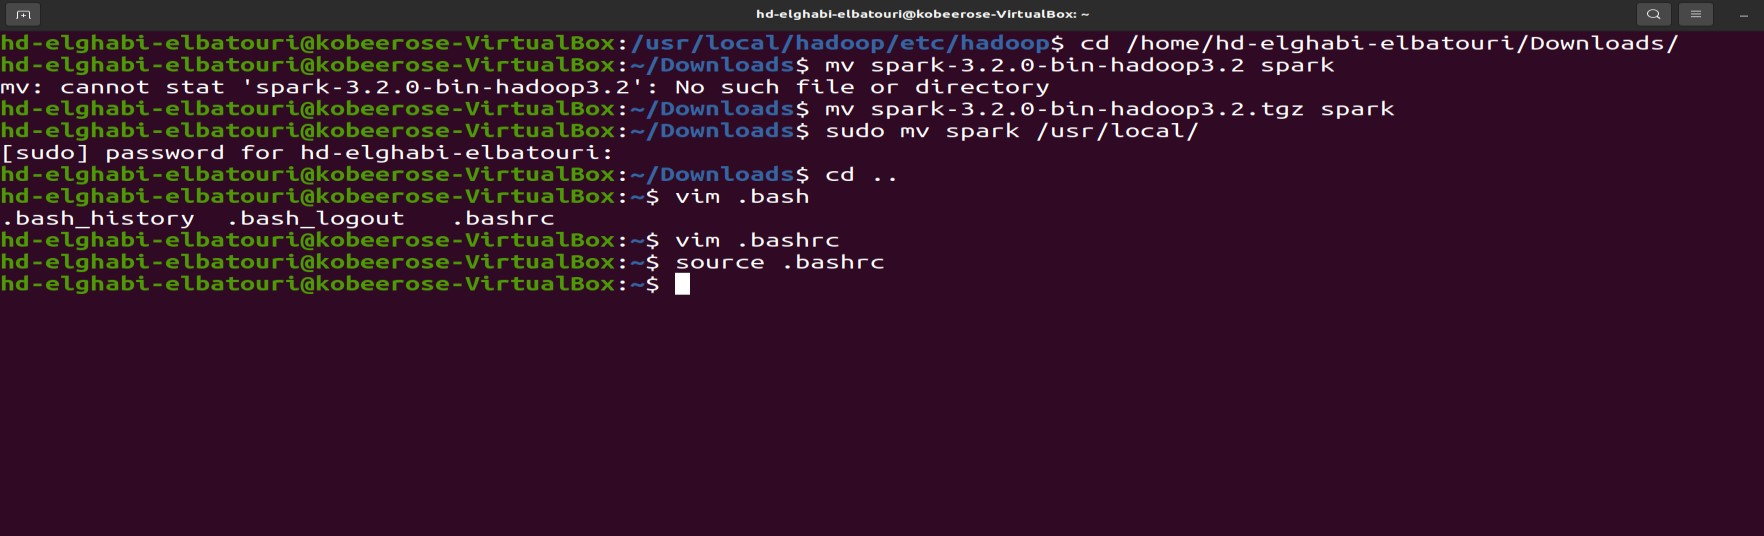
\includegraphics[width=1\linewidth]{Big_Data/Spark/Spark Installation & Configuration/Extracting Spark.jpg} 
\end{center} 
\caption{caption} 
\end{figure} 
\FloatBarrier

\section{Configure the PATH in the .bashrc}

\par modify the PATH by adding the path where the bin of spark exists.
\\
\begin{figure}[!htb] 
\begin{center} 
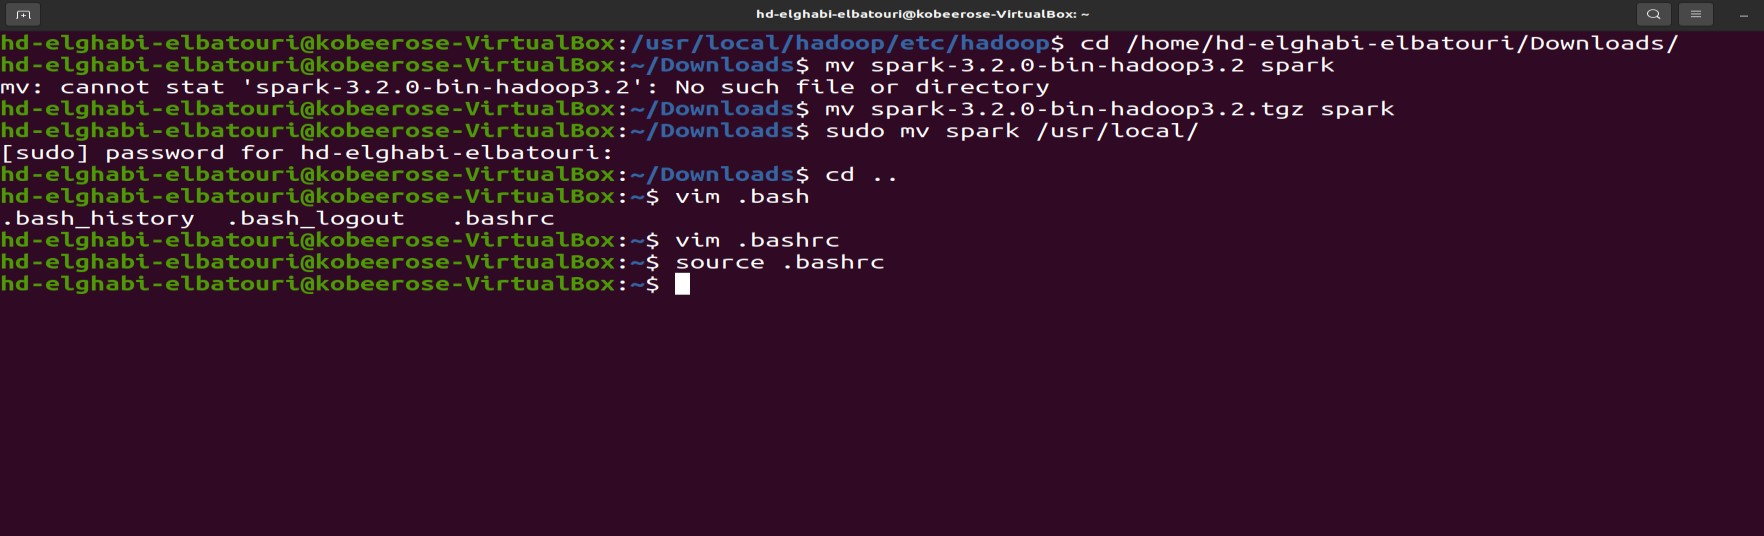
\includegraphics[width=1\linewidth]{Big_Data/Spark/Spark Installation & Configuration/.bashrc config.jpg} 
\end{center} 
\caption{caption} 
\end{figure} 
\FloatBarrier

\section{Installing Python}


\par Let's install python on our machine.
\\
\begin{figure}[!htb] 
\begin{center} 
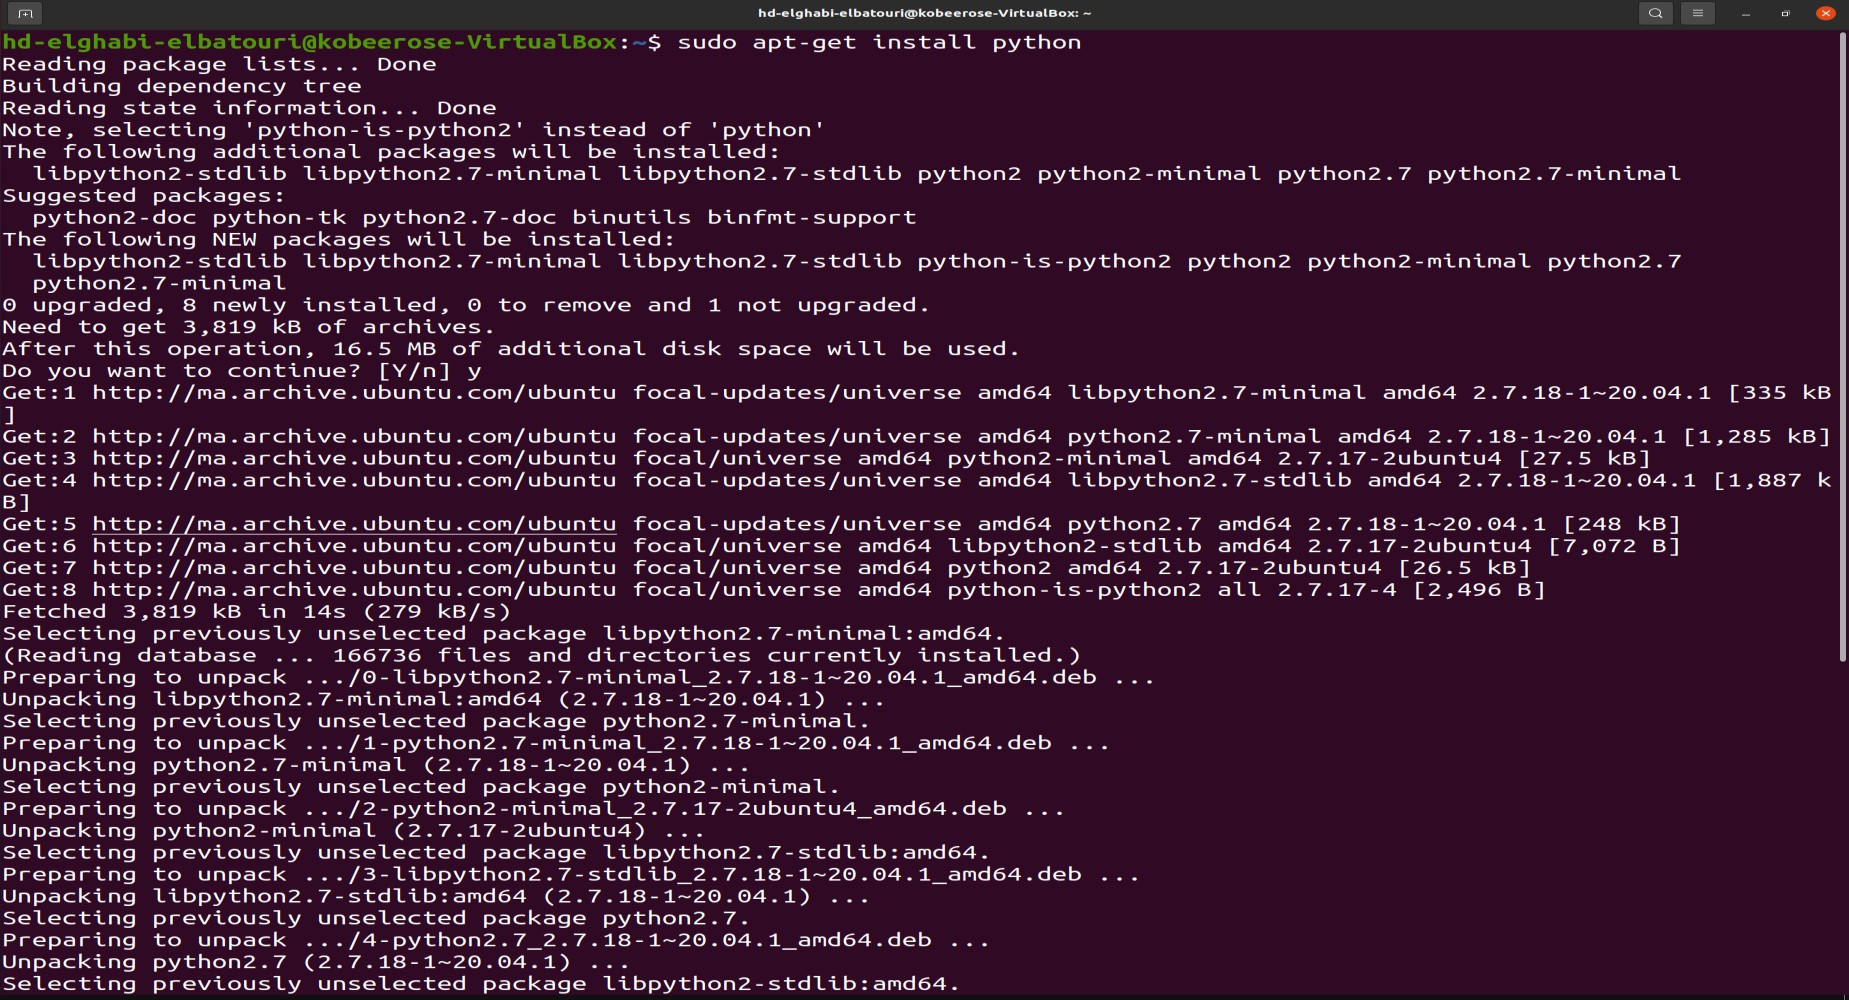
\includegraphics[width=1\linewidth]{Big_Data/Spark/Spark Installation & Configuration/Installing Python.jpg} 
\end{center} 
\caption{caption} 
\end{figure} 
\FloatBarrier


\par Accessing the Python terminal for Spark.
\\
\begin{figure}[!htb] 
\begin{center} 
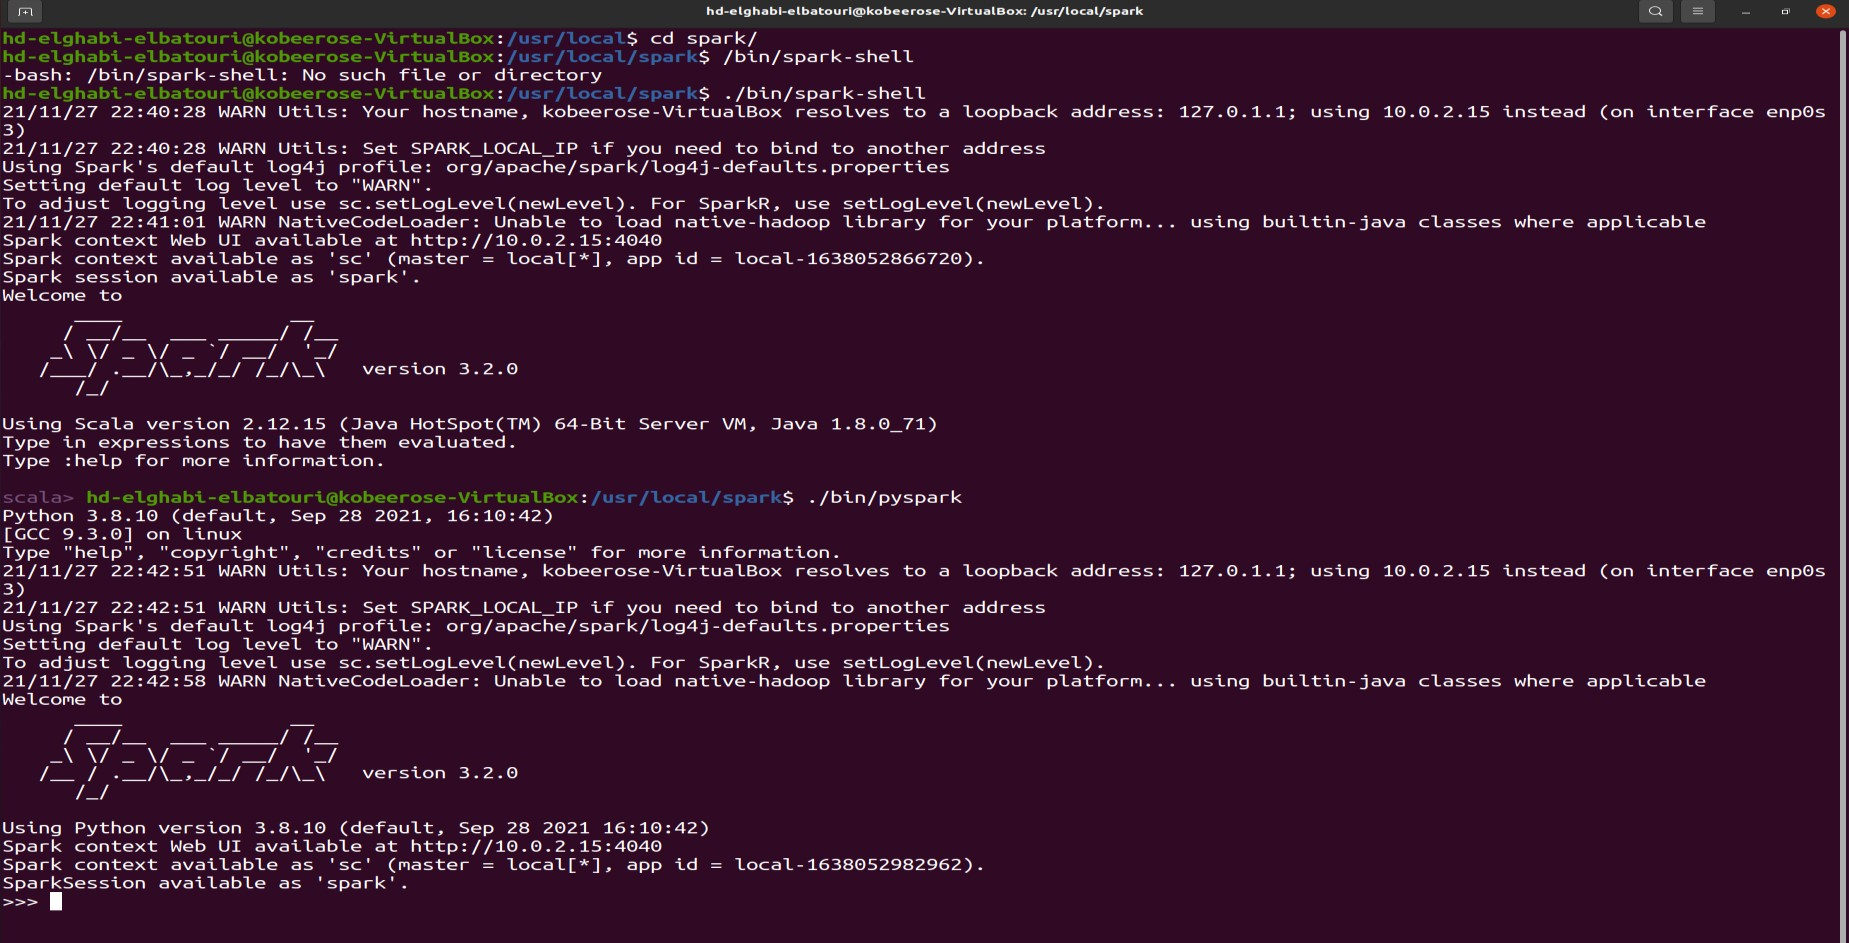
\includegraphics[width=1\linewidth]{Big_Data/Spark/Spark Installation & Configuration/spark-shell & pyspark.jpg} 
\end{center} 
\caption{caption} 
\end{figure} 
\FloatBarrier



\end{spacing}